\documentclass[12pt]{article}
\usepackage[margin=2.5cm]{geometry}
\usepackage{polski}
\usepackage[utf8]{inputenc}
\usepackage{qtimes}
\usepackage{setspace}
\usepackage{amssymb}
\usepackage{graphicx}

\graphicspath{ {images/} }
\doublespacing

\title{O zachowaniach społecznych szczurów}
\author{Marcin Parafiniuk}
\date{\today}

\newcommand{\apaartykul}[6]{#1 (#2). #3. \textit{#4}, \textit{#5} s. #6}

\begin{document}

\maketitle

\tableofcontents

\pagebreak

\section{Wstęp}

Szczury to zwierzęta, które towarzyszą człowiekowi od dawna. Szczur, tak jak wróbel czy gołąb, jest jednym z gatunków, które świetnie czują się w środowisku zurbanizowanym. W osiemnastowiecznej Europie szczur był jednym z najpopularniejszych szkodników gnieżdżących się w miastach. Stanowiło to na tyle duży problem, że powstał cały poddział przemysłu, trudniący się zwalczaniem tychże szkodników. Szczurołapowie, oprócz zarabiania na zwalczaniu gryzoni, obławiali się na sprzedawaniu szczurzego mięsa, lub na tzw. szczurzych igrzyskach.

Szczurze igrzyska polegały na tym, że złapane gryzonie wpuszczało się na arenę razem z jednym terrierem. Zebrani naokoło widzowie mogli zakładać się o to, jak szybko pies zabije wszystkie szkodniki. Ten całkiem popularny sport, zanim został zakazany, przyciągał tłumy. Psy które zabijały szczury najszybciej, zostawały lokalnymi celebrytami, ich właścicielowie szybko się wzbogacali. Niedługo okazało się, że szczurołapowie nie nadążają z łapaniem gryzoni na potrzeby igrzysk i organizatorzy takich wydarzeń byli zmuszeni zainwestować w hodowlę szczurów.

Hodowle radykalnie różniły się warunkami od tego do czego gryzonie były przyzwyczajone w naturalnym środowisku, miejskim, czy leśnym. Dobór naturalny został zakłócony, często miał miejsce chów wsobny. Wskutek tego wśród szczurów zaczęły pojawiać się mutacje. W ten sposób pojawiły się albinosy i osobniki o tzw. umaszczeniu kapturowym. Ludzie zainteresowali się różnicami pomiędzy zwykłymi szczurami, a dziwnymi białymi wyjątkami pochodzącymi z hodowli. W 1828 pierwszy raz szczur albinos wziął udział w eksperymencie dotyczącym poszczenia. Podczas następnych 30 lat szczury były używane jako obiekty doświadczalne w kolejnych eksperymentach i w końcu szczur laboratoryjny został udomowiony ze względów naukowych.

Szczury są droższe w utrzymaniu niż myszy, dlatego głównym obiektem badań laboratoryjnych wciąż pozostają mniejsze gryzonie. Jednak w niektórych polach szczury zdecydowanie przodują w statystykach nad swoim mniejszym krewniakiem. Takim polem jest między innymi psychologia, jako że szczury charakteryzują się silniejszym instynktem stadnym niż myszy, są też bardziej inteligentne.

\pagebreak

W środowisku naturalnym stado szczurów może liczyć nawet 200 osobników. Jasne jest, że tak duże kolonie nie mogą istnieć bez jakiegoś sposobu, na który osobniki mogą się ze sobą porozumiewać. Zafascynował mnie ten temat. W jaki sposób owe złożone, inteligentne zwierzęta utrzymują jedność stada? Jak skomplikowane są komunikaty, które sobie nawzajem przekazują? Czy ze szczurem da się w jakiś sposób "porozmawiać" - a jeśli tak, to o czym? Odpowiedzi na te pytania, chociażby niepełne, postarałem się zawrzeć w tej pracy.

\section{Biochemiczne podłoże zachowań społecznych szczurów}

\subsection{Opioidy}

Pomysł na to, że endogenne opioidy regulują zachowania społeczne pochodzi od tego, że uzależnienie od opiatów i potrzeba kontaktu z innymi szczurami mają podobne charakterystyki. W obu przypadkach zachodzi faza początkowego przywiązania i faza budowania tolerancji, podobne są też objawy odstawienne (Panksepp, J., Herman, B.H., Conner, R., Bishop, P., Scott, J.P., 1978; Panksepp, J., Herman, B.H., Vilberg, T., Bishop, P., DeEskinazi, F.G., 1980). Wykazano też, że podawanie morfiny zmniejsza częstotliwość ultradźwiękowych wokalizacji wywołanych przez izolację dwutygodniowych szczurów od matki, podczas gdy młode w tym wieku wciąż powinny być karmione piersią i ich relacja z matką jest bardzo bliska (Carden, S.E., Barr, G.A., Hofer, M.A., 1991).
Jednak u młodych szczurów dawki, które redukują ultradźwiękowe wokalizacje, wpływają również na ogólne zmniejszenie aktywności. Młode gryzonie różnią się zarówno od starszych przedstawicieli tego samego gatunku jak i od innych gatunków zdecydowanie większą wrażliwością na opioidy podczas dwóch pierwszych tygodni życia, prawdopodobnie ze względu na większą przenikalność bariery krew-mózg (Banks, W.A., Kastin, A.J., 1985).

Badania dotyczące antagonistów, hamujących wydzielanie endogennych pochodnych morfiny również wskazują na specyfikę opioidów w regulowaniu zachowań społecznych. Nalokson i naltrekson blokują pozytywny wpływ opioidów na ilość wokalizacji. Podane same (bez równoważącej dawki opioidów) często zwiększają efekt społecznej izolacji (Panksepp, J. i in., 1980).

Istnieją badania, które wskazują na to, że niektóre bodźce społeczne, na przykład bycie karmionym piersią, również wiąże się z wydzielaniem endogennych opioidów. U nowonarodzonych szczurów występuje zmniejszenie wrażliwości na dotykowe bodźce zewnętrzne podczas karmienia piersią. Ten efekt jest blokowany przez podanie małemu szczurowi opioidowego antagonisty, wskazując na to że reakcja na bycie karmionym piersią obejmuje wydzielanie endogennych opioidów (Smotherman, W.P., Robinson, S.R., 1992).

Podczas okresu dojrzewania szczury, tak jak praktycznie wszystkie gatunki ssaków bawią się w gonitwy i przepychanki. Wykazano, że zasadniczym celem takiego zachowania są interakcje somatosensoryczne (Siviy, S.M. and Panksepp, J., 1987). Badania przy pomocy subtraktywnej autoradiografii wykazały że szczurze zabawy skutkują wydzielaniem endogennych opioidów, oraz że podanie szczurom naloksonu wpływa na zmniejszenie poziomu tych zabaw (Panksepp, J., Bishop, P., 1987; J. Panksepp, S.M. Siviy, L.A. Normansell, 1985).  Po podaniu naloksonu młode po prostu czują, że gonitwa i przepychanki nie dają im już takiej frajdy.

\subsection{Oksytocyna}

Wykazano, że podanie oksytocyny zmniejsza częstotliwość ultradźwiękowych wokalizacji u młodych szczurów (Insel, T.R. and Winslow, J.T., 1991). To odkrycie sugeruje, że oksytocyna może mieć zasadnicze znaczenie w subiektywnym odczuciu "spokoju", który młode okazują podczas interakcji z matką i innymi szczurami. Inne badanie z kolei wykazało że podanie antagonisty oksytocyny blokuje efekt kojarzenia zapachu matki z przyjemnymi doznaniami u młodych szczurów (Nelson, E. and Panksepp, J., 1996).

W kolejnym badaniu młode we wczesnej fazie rozwoju zostawały kilkukrotnie poddawane izolacji od matki. Okazało się, że ich receptory oksytocyny w hipokampie zostały zredukowane (Noonan, L.R., Caldwell, J.D., Li, L., Walker, C.H., Pedersen, C.A. and Mason, G.A., 1994). Chociaż dokładne znaczenie tego odkrycie jest niejasne, na pewno wskazuje ono na dużą rolę oksytocyny w interakcjach społecznych młodych szczurów z matką.

\pagebreak

Prawdopodobnie tak jak w przypadku opioidów, oksytocynowe neurony są aktywowane przez jakikolwiek społeczny kontakt fizyczny. Eksperyment szwedzkich naukowców wykazał, że poziom oksytocyny w krwi i płynie mózgowo-rdzeniowym wzrasta podczas głaskania lub delikatnego ogrzewania szczura (Uvnas-Moberg, K., Bruzelius, G., Alster, P. Lundeberg, T., 1993).

\subsection{Wazopresyna}

Chociaż nie tak popularna w literaturze jak oksytocyna, wazopresyna również może pełnić istotną rolę w komunikacji szczurów. Podanie tego hormonu, podobnie jak w przypadku poprzednio wymienionych substancji, zmniejsza częstotliwość ultradźwiękowych wokalizacji u młodych oddzielonych od matki (Winslow, J.T., Insel, T.R., 1993). Co więcej, u szczepu Brattleboro, charakteryzującego się naturalnym deficytem wazopresyny, wykazano zmniejszoną reakcję u młodych na zapach matki (Nelson, E., Bird, L., Deak, T., Vaningan, M. Panksepp, J., 1995).

\section{Zachowania empatyczne i potrzeba społeczna}

\subsection{Altruizm}

U pewnego procentu naszego społeczeństwa możemy zaobserwować zachowania altruistyczne. Są to zachowania nie przynoszące bezpośrednio zysku osobie je wykonującej, lecz wykonywane by pomóc komuś innemu. Istnienie tego zjawiska wynika z tego, że jesteśmy zdolni do empatii -- współodczuwania czyjegoś dyskomfortu. To wytwarza motywację do bezinteresownej pomocy. Jednak czy takie zjawisko jest czymś charakterystycznym wyłącznie dla ludzi, czy może jest ewolucyjnie uzasadnionym mechanizmem funkcjonującym również u innych wysoce społecznych gatunków -- na przykład szczurów? Na to pytanie spróbowali znaleźć odpowiedź Bartal, Decety i Mason (2011).

Eksperyment, który przeprowadzili składał się z kilku faz. Na początku szczury zostały podzielone na pary i mieszkały ze sobą w klatkach przez dwa tygodnie. Ten element został wprowadzony po to, żeby szczury mogły się przyzwyczaić do siebie nawzajem, ale także po to żeby umożliwić im wytworzenie pomiędzy sobą pewnej więzi której istnienie będzie mogło później motywować do działań altruistycznych.

Następnie pary były umieszczane na arenie testowej. Na środku areny znajdowała się mała klatka, w której był uwięziony jeden osobnik. Drugi był puszczony wolno. Wolny szczur miał możliwość uwolnienia swojego kolegi poprzez przyłożenie pewnej siły do drzwi. Jeśli to uwolnienie nie następowało, eksperymentator otwierał drzwi do połowy, żeby uświadomić szczurom działanie mechanizmu i uniknąć stworzenia wrażenia sytuacji bez wyjścia.

W sytuacji kontrolnej szczur zostawał wpuszczany na arenę, ale w klatce zamiast jego współtowarzysza znajdował się pluszak o kształcie szczura, lub klatka była pusta. W drugiej sytuacji kontrolnej szczury z pary były oddzielone od siebie perforowanym materiałem i u jednego z nich znajdowała się pusta klatka. Głowy wolno puszczonych szczurów były oznaczane markerem po to, by móc kontrolować w którym miejscu areny statystycznie najwięcej spędzają czasu. Badanie trwało 12 dni.

Wolne szczury krążyły dookoła klatki, próbując w niej kopać i ją gryźć oraz utrzymywały kontakt z uwięzionym kolegą przez otwory w plastiku. Nauczyły się otwierać drzwi i uwalniać towarzysza średnio w 6.9 ($\pm$2.9) dnia. Spędzały istotnie więcej czasu w pobliżu klatki w środku areny, poruszały się szybciej i były dużo bardziej aktywne niż szczury kontrolne. Stąd wniosek, iż testowane szczury były zmotywowane do ruchu i działania w obecności uwięzionego pobratymca.

Podczas kolejnych sesji w sytuacji z więźniem proporcja szczurów, które otwierały klatkę rosła, a czas do otwarcia drzwi zmniejszał się, co dowodzi uczenia się. Istotnie więcej szczurów (23/30), niż w sytuacji kontrolnej (5/40) zdecydowały się otworzyć klatkę chociaż raz podczas trwania całego eksperymentu. U wolnego szczura podczas otwierania klatki aktywność zdecydowanie się zwiększała, co sugeruje że zdarzenie otwarcia klatki było dla niego znaczące. Na początku dźwięk i ruch otwieranych drzwi powodowały, że wolny szczur zastygał w bezruchu ze strachu, jednak w kolejnych dniach efekt zastygania wygasał, co sugeruje że otwieranie drzwi było efektem celowego działania i szczur spodziewał się, jaki efekt osiągnie.

W kolejnej części eksperymentu szczury musiały zmierzyć się z nowym zadaniem. Tym razem klatka ustawiona była tak, że gdy drzwi zostały otwarte przez wolnego szczura, więzień musiał wybiec do oddzielonego fragmentu wybiegu, niedostępnego dla wolnego szczura. Takie ustawienie klatki miało na celu zbadanie, czy wolny szczur uwalnia kolegę tylko po to, żeby się z nim pobawić, czy ma też na uwadze jego dyskomfort psychiczny i uwolni go tylko po to żeby mu pomóc. Okazało się, że niezależnie od zmienionej sytuacji szczury wciąż otwierają klatkę. To wskazuje na to, że oczekiwanie nagrody w postaci kontaktu społecznego nie jest konieczne, by szczur wykonał wysiłek mający na celu dobro drugiego szczura.

W kolejnej, ostatniej już części eksperymentu wolny szczur miał do wyboru klatkę w której jest uwięziony kolega i klatkę, w której znajdował się szczurzy przysmak -- czekolada. W sytuacji kontrolnej wolny szczur wybierał między pustą klatką a tą ze słodkościami. Podczas testu tak samo często była otwierana klatka z więźniem, jak i z czekoladą, podczas gdy w sytuacji kontrolnej zdecydowanie częściej był wybierany przysmak. Wyniki pokazują, że uwalnianie uwięzionego towarzysza jest dla szczurów podobnie ważne jak dostanie się do ulubionego jedzenia. Dodatkowo, pomimo tego, że wolny szczur mógł zjeść całą czekoladę sam, w ponad połowie przypadków dzielił się on zdobytym jedzeniem z uwolnionym kolegą.

Podsumowując, badania pokazały że szczury wykazują działania altruistyczne gdy widzą swojego pobratymca doświadczającego niefizycznego dyskomfortu psychicznego i podejmują świadome, celowe działania w celu skrócenia dyskomfortu innego szczura. Co więcej, to zachowanie wystąpiło pomimo braku treningu oraz w konfrontacji z atrakcyjnym przysmakiem.

\subsection{Kontakt społeczny jako alternatywa dla opiatów}

\subsubsection{Tło historyczne}

Po drugiej wojnie światowej były prowadzone badania nad narkotykami, w szczególności opiatami. Negatywny wpływ tych substancji na umysł człowieka był jasny, potrzeba było jednak konkretnych, naukowych badań żeby to potwierdzić. Takie właśnie badania prowadzili Nichols, Headlee, oraz Coppock (1956), Stolerman i Kumar (1973), Khavari i Risner (1973) oraz Ternes (1975). Wszyscy oni przyjmowali podobną metodologię. Zamykali szczura w klatce i dawali mu możliwość przyjmowania opiatów w jakiś sposób -- przez udostępnienie wody zanieczyszczonej opiatem, bezpośrednie wprowadzenie substancji do krwiobiegu itp. W innym wariancie najpierw szczur był uzależniany od narkotyku, a potem dostawał wybór -- mógł albo kontynuować przyjmowanie opiatów albo nie. W obu przypadkach skutek był podobny -- szczur się uzależniał od badanej substancji, czasami nawet ze skutkiem śmiertelnym i usatysfakcjonowani badacze publikowali badania że opiaty są złe.

Pomyślmy jednak przez chwilę jak czuje się ten szczur. Jedyna rozrywka jaką ma w tej ciemnej, samotnej klatce to narkotyk. Zostaje wprowadzony w uzależnienie i nie ma żadnej motywacji żeby z tym walczyć. Nie ma żadnych perspektyw, nikt na niego nie czeka. Jedyne co jest to ciemna klatka i nałóg. W takich warunkach niesamowitej siły woli wymagałoby utrzymanie abstynencji, lub wręcz wychodzenie z uzależnienia.

\subsubsection{Rat Park}

Do podobnego wniosku doszli naukowcy z wydziału psychologii na Simon Fraser University, prowadząc swoje badania (Bruce K. Alexander, Robert B. Coambs, Patricia F. Hadaway, 1978; Alexander, B.K., Beyerstein, B.L., Hadaway, P.F., Coambs, R.B., 1981). Skonstruowali więc swój eksperyment nieco inaczej. Tym razem były dwie grupy szczurów -- jedna, jak poprzednio, mieszkała w samotnych klatkach, ale druga przebywała w tzw Rat Parku. Był to spory obszar, w którym szczury ze sobą przebywały, mogły się bawić, łączyć w pary, środowisko było urozmaicone różnymi przedmiotami, zasadniczo było tam wszystko czego szczurza dusza mogła zapragnąć.

Analogicznie jak w niektórych poprzednich eksperymentach, obie grupy szczurów na początku przez pewien okres czasu dostawały tylko morfinę, a potem miały wybór -- morfina lub woda. I tak samo jak w poprzednich badaniach, kiedy przyszedł okres wyboru grupa kontrolna przebywająca w samotnych klatkach konsekwentnie została przy morfinie aż do uzależnienia fizycznego. Jednak zgodnie z przewidywaniem badaczy grupa mieszkająca w Rat Parku zrezygnowała z morfiny jak tylko pojawiła się czysta woda.

Okazało się, że szczury preferują swoje własne towarzystwo niż otępianie się narkotykiem. Zresztą, jak wspomniałem już wcześniej w tej pracy, a czego naukowcy z Simon Fraser University mogli nie wiedzieć, endogenne opiaty są zasadniczym elementem biochemicznej odpowiedzi na społeczne stymulanty. W związku z tym gryzonie, których społeczna potrzeba była zaspokojona miały zmniejszoną tendencję do konsumpcji opiatów egzogennych. Za to te, które bardzo potrzebowały kontaktu z innymi przedstawicielami własnego gatunku i w związku z tym poziom endogennych opiatów był u nich zaniżony, w zrozumiałej konsekwencji spożywały więcej morfiny aż do uzależnienia fizycznego.

\subsection{Wpływ relacji ze społecznością na rozwój}

Hebb (1947) pokazał, że szczury hodowane jako jego zwierzątka domowe mają lepsze wyniki na teście inteligencji Hebba-Williamsa niż grupa kontrolna hodowana w laboratorium, ale to był tylko początek. Od tamtego czasu zdobyto konkretne dowody na to, że izolacja młodych od szczurzego społeczeństwa ma długotrwałe negatywne skutki w rozwoju ich mózgu. W szczególności stwarza to predyspozycje do schizofrenii i depresji, ale także do zaburzonego rozwoju hipokampu.

U szczura niektóre struktury mózgu (m.in. właśnie hipokamp) wykształcają się w pełni nawet 35-40 dni po urodzeniu (Lanier, Issacson, 1977). To powoduje, że mózg jest podatny na skutki manipulacji środowiskiem na wczesnym etapie rozwoju. Bazując na tych obserwacjach Lapiz i in. (2003) przeprowadzili eksperyment mający zbadać skalę tego zjawiska.

Szczury w wieku $\geq$21 dni zostały w grupie testowej oddzielone od reszty swojej szczurzej rodziny na okres 6-8 tygodni. W grupie kontrolnej szczury były pozostawione przy matce i rodzeństwie. Następnie przeprowadzane były różne testy sprawnościowe mające na celu sprawdzić, jak sposób hodowania szczura wpłynął na wynik osiągany przez osobnika.

Jednym z takich testów był labirynt wodny. Test ten ma dwie fazy. Podczas pierwszej szczur jest wpuszczany do pojemnika z wodą. W wodzie znajduje się platforma, do której jeśli szczur dopłynie, zostanie wzięty z powrotem do bezpiecznego środowiska. Ta faza ma na celu nauczenie szczura tego, że powinien szukać platformy i gdzie ona się znajduje. W drugiej fazie testu natomiast poziom wody jest zwiększany tak, że platforma staje się niewidoczna. Szczur wpuszczony do pojemnika, pomimo braku sygnału wzrokowego, powinien podpłynąć do miejsca, w którym wie że czeka go ratunek, znaleźć znajdującą się tuż pod powierzchnią wody platformę i się na nią wydostać. Test ten ma na celu sprawdzenie jak szczur radzi sobie w stresującej sytuacji, jego umiejętność uczenia się i pamięć.

Inny test wyglądał następująco: najpierw warunkowano szczurom CER (conditioned emotional response -- wyouczona reakcja emocjonalna) na przebywanie w pewnym pomieszczeniu. Robiono to w taki sposób, że klatka, do której szczury miały sobie wytworzyć reakcję emocjonalną miała w podłodze położone pręty, przez które był puszczany impuls elektryczny, nieprzyjemny dla gryzoni. Naturalnie więc po pewnym czasie przebywające w tej klatce osobniki zaczynają się jej bać. Następnie przez mierzenie poziomu dopaminy mierzy się siłę i czas reakcji emocjonalnej szczura na bodziec, na który został uwarunkowany.

W obu testach gryzonie, które były społecznie izolowane we wczesnej fazie rozwoju radziły sobie gorzej. W teście labiryntu wodnego dłużej im zajmowało odnalezienie platformy, nie mogły się skupić, gorzej też funkcjonowała pamięć. W teście elektrycznej podłogi reakcja dopaminergiczna była silniejsza i dłużej się utrzymywała. Dodatkowo, pomiary ogólnej aktywności (nie tylko podczas testów) wykazały, że szczury izolowane ruszają się więcej i bardziej dynamicznie. Można z tych wyników wyciągnąć wniosek, że społeczna izolacja za młodu wykształciła w szczurach większą podatność na stres i skłonność do przeżywania napięcia nawet w sytuacjach, którego tego nie wymagają.

\section{Komunikacja werbalna}

\subsection{Informacje ogólne}

Żeby rozważać szczurzą komunikację, zdefiniujmy najpierw co to pojęcie oznacza. Do szczurów dociera wiele bodźców z zewnątrz. Niektóre z nich pochodzą od pobratymców, niektóre od środowiska. Niektóre są w stanie wpływać na motywację lub stan wiedzy szczura, inne nie. Komunikacją nazwiemy proces przekazywania informacji. Ze strony nadawcy więc jest to rozmyślne, adresowane emitowanie bodźca przez jednego osobnika, które ma na celu wpływ na motywację lub wiedzę o świecie innego osobnika. Ze strony odbiorcy natomiast jest to otrzymanie oraz przetworzenie tego bodźca w taki sposób, że osiąga on cel zadany przez nadawcę. Tylko wtedy jeśli po obu stronach doszło do zajścia opisanych zjawisk, możemy mówić że zaszła pomiędzy nimi komunikacja.

Jak pisze Brudzynski (2005), u szczurów komunikaty werbalne najczęściej dotyczą ogólnej sytuacji zewnętrznej, stanu psychicznego (motywacji), a nie konkretnych przedmiotów lub ich własności. Tak więc nie dość, że szczurom brakuje zdolności artykulacji istotnie różniących się od siebie głosek, w ich "języku" nie znajdziemy również gramatyki, czy syntaktyki. Komunikaty o tym samym znaczeniu potrafią też istotnie się różnić. Pomimo to, szczury spójnie odpowiadają na sygnały wokalne pobratymców i potrafią rozumieć semiotyczną istotę przekazu.

Zaobserwowano u szczurów komunikację dotyczącą kilku zasadniczych aspektów:
\begin{itemize}
    \item funkcja lokalizująca -- na przykład młode wydają dźwięk, żeby matka wiedziała gdzie się znajdują, matka im odpowiada żeby wiedziały, że wciąż jest w pobliżu
    \item przekaz zawierający walencję wewnętrznego stanu emocjonalnego nadawcy
    \item zwrócenie uwagi odbiorcy, lub zmobilizowanie go do jakiejś akcji która nie jest dokładnie wyrażona
    \item funkcja alarmująca informująca o zewnętrznym niebezpieczeństwie (wywołująca w odbiorcach na przykład zastygnięcie lub inne reakcje defensywne)
    \item przekazanie komunikatu nakazującego ucieczkę, wycofanie, lub rozpierzchnięcie się
    \item funkcja afiliacyjna, komunikat sygnalizujący chęć zbliżenia się do społeczności i kontaktu
    \item funkcja fatyczna, utrzymująca relację pomiędzy osobnikami i utrzymująca spójność grupy społecznej
\end{itemize}

W zależności od struktury akustycznej komunikatu i wywołanego zachowania, wokalizacja może być monosemiczna lub polisemiczna -- mieć jeden przekaz (jedno znaczenie w ludzkim języku), lub wiele. Mimo że niektóre komunikaty istotnie mają monosemiczne funkcje, najprawdopodobniej większość komunikatów gryzoni jest polisemiczna. Dodatkowo, szczurza komunikacja werbalna (w obecnym stanie wiedzy) wydaje się bardziej probablistyczna niż deterministyczna. Dalsze badania są niezbędne, by w pełni zrozumieć wielowymiarową strukturę semiotyczną szczurzych przekazów.

Szczurza wokalizacja jest zjawiskiem typowo społecznym i zazwyczaj zanika u dorosłych osobników w sytuacji gdy nie mają one kontaktu z innymi dorosłymi osobnikami. Jednak u młodych, podczas nieobecność matki częstość i natężenie wokalizacji zwiększa się. Spontaniczne komunikaty u dorosłych szczurów podczas izolacji pojawiają się dopiero w długotrwałej, stresującej sytuacji.

\subsection{Komunikaty o częstotliwości 22kHz}

Komunikaty alarmowe dorosłych szczurów pod względem częstotliwości mieszczą się w przedziale 18-32kHz z dość wąskim pasmem 1-6kHz i długim czasem trwania -- od 300 do 3400ms (Barfield, R. J., Geyer, L. A., 1975; Brudzynski, S. M., Bihari, F., Ociepa, D., Fu, X. W., 1993; Brudzynski, S. M., Ociepa, D., 1992). Te własności akustyczne są obserwowane w sytuacjach zagrożenia, niebezpieczeństwa, lub dyskomfortu. W szczególności relatywnie stała częstotliwościa dźwięku i długi czas trwania wydają się najważniejsze dla przekazania znaczenia tych wokalizacji. Kolejne badania wykazały, że dźwięki o tych charakterystykach generowane sztucznie również miały duży wpływ na zachowanie kolonii szczurów (Brudzynski, S. M., Chiu, E. M., 1995; Brudzynski S. M., 2001; Sales, G. D., 1991).

Powstaje pytanie jak szczury mogą wyrazić stopień zagrożenia. Największą wariancję widać zdecydowanie w długości wokalizacji. Najkrótsze i najdłuższe komunikaty różniły się między sobą więcej niż 195-krotnie (20ms -- 3940ms). Tak więc można postawić tezę, że ten parametr jest najwłaściwszy do wyrażania różnic w stopniu alarmu. Jednak bezpośrednie badanie relacji długości przekazu do stopnia zewnętrznego niebezpieczeństwa nie zostało jeszcze przeprowadzone. 

\subsection{Komunikaty o częstotliwości 50kHz}

Innym typem komunikatu są te emitowane zarówno przez młode jak i dorosłe szczury o częstotliwości w przedziale 35–72 kHz (Blanchard i in., 1993; Brudzynski, S. M., Pniak, A., 2002; Fu, X. W., Brudzynski, S. M., 1994; Kaltwasser M.-Th., 1990; Takahashi, L. K., Thomas, D. A., Barfield, R. J., 1983; Wintink, A. J., Brudzynski, S. M., 2001). Wokalizacje trwają krótko -- od 30 do 50 ms -- i mają wąskie pasmo 5-7kHz. Wyniki niektórych badań (w tym tych podanych wyżej) wskazują, że wszystkie z tych parametrów charakteryzują się podobną zmiennością -- największa i najmniejsza wartość różni się 4.8-krotnie dla długości, 4-krotnie dla częstotliwości i 4.6-krotnie dla pasma.

W tym typie wokalizacji natężenie komunikatu jest prawdopodobnie przekazywane po prostu przez ilość wydawanych dźwięków. Zaobserwowano, że ilość 50-kHz wokalizacji drastycznie rośnie w niektórych sytuacjach społecznych, podczas kiedy częstotliwość nie ulega istotnej zmianie. W sytuacji, kiedy szczury spodziewały się, że nastąpi kontakt społeczny, częstość komunikatu wzrosła 16-krotnie. Dodatkowym argumentem za tym, że to ilość wokalizacji odpowiada za natężenie przekazu jest to, że pasmo dźwięku jest raczej wąskie i niezmienne.

\ifx true false
t is, however, more
probable that the quantitative sign dimension is
simply coded in the number of calls emitted by rats
in this particular type of calls. A dramatic increase
in the number of 50-kHz calls was observed in
some social situations (Fig. 4) without any signifi-
cant increase in mean peak frequency (Brudzynski
and Pniak, 2002). The change from low to high
levels of calling, which was generated in anticipa-
tion of a social contact, changed on average by 16
times
\fi

\section{Podsumowanie}

Nie ulega wątpliwości, że szczury to stworzenia wysoce społeczne i inteligentne. W ich układach nerwowych zachodzą skomplikowane reakcje regulujące potrzebę społeczną oraz sposób przeżywania kontaktu z innymi szczurami. Substancje odpowiadające za regulacje tych procesów mają podobną rolę w układzie nerwowym człowieka, dlatego szczury mogą być dobrym obiektem do badań ludzkich mechanizmów i potrzeby społecznej.

Szczury wykazują też rozmyślne zachowania altruistyczne -- w pewnych sytuacjach są skłonne zainwestować swój wysiłek dla dobra drugiego szczura, nawet bez jasnego bezpośredniego zysku dla siebie. Kontakt społeczny jest dla nich na tyle ważny i satysfakcjonujący, że nawet mając do dyspozycji silne substancje odurzające nie decydują się na zażywanie ich w dużych ilościach o ile żyją blisko społeczności innych szczurów. I wreszcie kontakt społeczny jest dla nich niezbędny aby prawidłowo się rozwijać. Osobnik pozbawiony za młodu kontaktu z innymi szczurami w dorosłości będzie borykał się z zaburzeniami układu nerwowego.

Oprócz komunikatów niewerbalnych szczury mają też dość złożony sposób komunikacji werbalnej. Występują w nim różne przekazy z różnymi charakterystykami, służące różnym celom. Są one używane przez szczury żeby świadomie i celowo przekazywać innym szczurom pewne informacje lub motywować je do pewnych działań.

Szeroko pojęta nauka, ale w szczególności psychologia, wiele szczurom zawdzięcza. Nie bez powodu w Nowosybirsku znajduje się pomnik poświęcony tym dzielnym zwierzętom. Oglądając jednak wiele eksperymentów muszę przyznać że ciężko mi się na sercu robiło widząc jak szczury są rażone prądem, podtapiane, trute, rozcinane i maltretowane na wiele innych sposobów. Nie zapominajmy o tym, że za ruszającymi się wąsikami i bystro błyszczącymi oczkami kryje się także żywy, czujący umysł. Doprawdy okrutny jest ten, kto na widok takiego słodkiego pyszczka wciąż ma jakieś niecne zamiary!


\begin{center}
    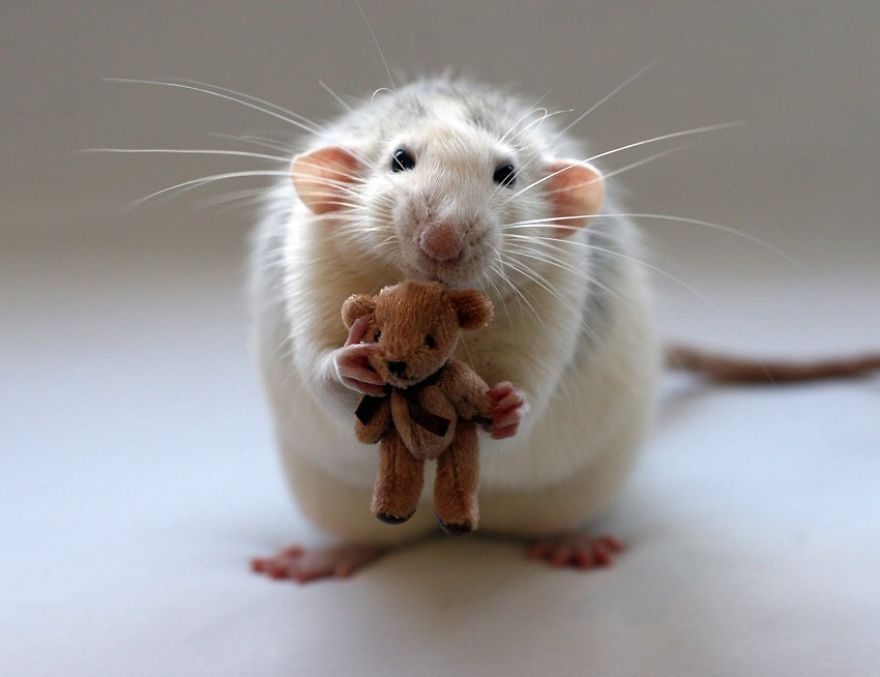
\includegraphics[width=18cm]{cuterat}
\end{center}

\pagebreak

\section{Bibliografia}
\apaartykul{Alexander, B.K., Beyerstein, B.L., Hadaway, P.F., Coambs, R.B.}{1981}{Effect of early and later colony housing on oral ingestion of morphine in rats}{Pharmacology Biochemistry and Behavior}{15}{571--576}

\apaartykul{Alexander, B.K., Coambs, R.B., Hadaway, P.F.}{1978}{The effect of housing and gender on morphine self-administration in rats}{Psychopharmacology}{58}{175--179}

\apaartykul{Banks, W.A., Kastin, A.J.}{1985}{Permeability of the blood-brain barrier to neuropeptides: The case for penetration}{Psychoneuro-endocrinology}{10}{385–399}

\apaartykul{Barfield, R. J., Geyer, L. A.}{1975}{The ultrasonic postejaculatory vocalization and the postejaculatory refractory period of the male rat}{J. Comp. Physiol. Psychol}{88}{732-734}

\apaartykul{Bartal, I. B. A., Decety, J., Mason, P.}{2011}{Empathy and pro-social behavior in rats}{Science}{334}{1427--1430}

\apaartykul{Blanchard, R. J., Yudko, E. B., Blanchard, C. D., Taukulis, H. K.}{1993}{High-frequency (35–70 kHz) ultrasonic vocalization  in  rats  confronted  with  anesthetized  conspecific: Effects  of  gepirone,  ethanol,  and  diazepam}{Pharmacol. Biochem. Behav.}{44}{313–319}

\apaartykul{Brudzynski, S. M., Bihari, F., Ociepa, D., Fu, X. W.}{1993}{Analysis of 22 kHz ultrasonic vocalization in laboratory rats: long and short calls}{Physiol. Behav}{54}{215-221}

\apaartykul{Brudzynski, S. M., Chiu, E. M.}{1995}{Behavioural responses of laboratory rats to playback of 22 kHz ultrasonic calls}{Physiol. Behav}{57}{1039-1044}

\apaartykul{Brudzynski, S. M., Ociepa, D.}{1992}{Ultrasonic vocalization of laboratory rats in response to handling and touch}{Physiol. Behav}{52}{655-660}

\apaartykul{Brudzynski, S. M., Pniak, A.}{2002}{Social contacts and production of 50 kHz short ultrasonic calls in adult rats.}{J. Comp. Psychol}{116}{73–82}

\apaartykul{Brudzynski, S. M.}{2001}{Pharmacological and behavioral characteristics of 22 kHz alarm calls in rats}{Neurosci. Biobehav. Rev.}{25}{611-617}

\apaartykul{Brudzynski, S. M.}{2005}{Principles of rat communication: quantitative parameters of ultrasonic calls in rats}{Behavior genetics}{35}{85-92}

\apaartykul{Carden, S.E., Barr, G.A., Hofer, M.A.}{1991}{Differential effects of specific opioid receptor agonists on rat up isolation calls}{Behav. Brain Res.}{62}{17–22}

\apaartykul{Fu, X. W., Brudzynski, S. M.}{1994}{High-frequency ultrasonic vocalization induced by intracerebral glutamate in rats}{Pharmacol. Biochem. Behav}{49}{835–841}

\apaartykul{Hebb, D. O.}{1947}{The effects of early experience on problem solving at maturity}{Am. Psychol.}{No. 2}{306--307}

\apaartykul{Insel, T.R., Winslow, J.T.}{1991}{Central administration of oxytocin modulates the infant rat’s response to social isolation}{Eur. J. Pharmacol.}{203}{149–152}

\apaartykul{Kaltwasser, M.-Th.}{1990}{Acoustic signalling in the black rat (Rattus rattus)}{J. Comp. Psychol.}{104}{227–23}

\apaartykul{Khavari, K. A., Risner, M. E.}{1973}{Opiate dependence produced by ad libitum drinking of morphine in water, saline, and sucrose vehicles}{Psychopharmacologia (Bed.)}{30}{291--302}

\apaartykul{Lanier, L. P., Issacson, R. L.}{1977}{Early developmental changes in the locomotor response to amphetamine and their relation to hippocampal function}{Brain Res.}{No. 126}{567–575}

\apaartykul{Lapiz, M. D. S., Fulford, A., Muchimapura, S., Mason, R., Parker, T., Marsden, C. A.}{2003}{Influence of postweaning social isolation in the rat on brain development, conditioned behavior, and neurotransmission}{Neuroscience and behavioral physiology}{33}{13-29}

\apaartykul{Nelson, E., Bird, L., Deak, T., Vaningan, M., Panksepp, J.}{1995}{Social behavior in the young, vasopressin deficient Brattleboro rat}{Soc. Neurosci. Abstr.}{20}{366}

\apaartykul{Nelson, E., Panksepp, J.}{1996}{Oxytocin mediates acquisition of maternally associated odor preference in preweanling rat pups}{Behav. Neurosci.}{110}{1–10}

\apaartykul{Nichols, J. R., Headlee, C. P., Coppock, H. W.}{1956}{Drug addiction. I. Addiction by escape training}{J. Am. Pharm. Assoc.}{45}{788--791}

\apaartykul{Noonan, L.R., Caldwell, J.D., Li, L., Walker, C.H., Pedersen, C.A., Mason, G.A.}{1994}{Neonatal stress transiently alters the development of hippocampal oxytocin receptors}{Dev. Brain Res.}{80}{115–120}

\apaartykul{Panksepp, J., Bishop, P.}{1981}{An autoradiographic map of (3H) diprenorphine binding in rat brain: Effects of social interaction}{Brain Res. Bull.}{7}{405–410}

\apaartykul{Panksepp, J., Herman, B.H., Conner, R., Bishop, P., Scott, J.P.}{1978}{The biology of social attachments: opiates alleviate separation distress}{Biol. Psychiat.}{13}{607–613}

\apaartykul{Panksepp, J., Herman, B.H., Vilberg, T., Bishop, P., DeEskinazi, F.G.}{1980}{Endogenous opioids and social behavior}{Neurosci. Biobehav. Rev.}{4}{473–48}

\apaartykul{Panksepp, J., Siviy, S.M., Normansell, L.A.}{1985}{Brain opioids and social emotion, in: M. Reite, T. Fields (Eds.)}{The Psychobiology of Attachment and Separation}{}{3-49}

\apaartykul{Sales, G. D.}{1991}{The effect of 22 kHz calls and artificial 38 kHz signals on activity in rats}{Behav. Processes}{24}{83-93}

\apaartykul{Siviy, S.M., Panksepp, J.}{1987}{Sensory modulation of juvenile play in rats}{Dev. Psychobiol.}{20}{39–55}

\apaartykul{Smotherman, W.P., Robinson, S.R.}{1992}{Kappa opioid mediation of fetal responses to milk}{Behav. Neurosci.}{106}{396–407}

\apaartykul{Stolerman, I. P., Kumar, R.}{1973}{Preferences for morphine in rats: validation of an experimental model of dependence}{Psychopharmacologia (Berl.)}{17}{137--150}

\apaartykul{Takahashi, L. K., Thomas, D. A., Barfield, R. J.}{1983}{Analysis of ultrasonic vocalizations emitted by residents during aggressive encounters among rats (Rattus norvegicus)}{J. Comp. Psychol.}{97}{207–212}

\apaartykul{Ternes, J. W.}{1975}{Induced preference for morphine in rats}{Bull. Psychon. Soc.}{5}{315--316}

\apaartykul{Uvnas-Moberg, K., Bruzelius, G., Alster, P., Lundeberg, T.}{1993}{The antinociceptive effect of non-noxious sensory stimulation is mediated partly through oxytocinergic mechanisms}{Acta Physiol. Scand.}{149}{199–204}

\apaartykul{Winslow, J.T., Insel, T.R.}{1993}{Effects of central vasopressin adminis-tration to infant rats}{Eur. J. Pharmacol.}{233}{101–107}

\apaartykul{Wintink, A. J., Brudzynski, S. M.}{2001}{The related roles of dopamine and glutamate in the initiation of 50-kHz ultrasonic calls in adult rats}{Pharmacol. Biochem. Behav}{70}{317–323}

\end{document}